\hbadness=10000 \vbadness=10000
\documentclass[journal,12pt,twocolumn]{IEEEtran}
%
\usepackage{setspace}
\usepackage{textcomp}
\usepackage{gensymb}
\usepackage{xcolor}
\usepackage{caption}
\usepackage{polynom}
\usepackage{enumitem}
%\usepackage{keyval}
%\usepackage{subcaption}
%\doublespacing
\singlespacing

%\usepackage{graphicx}
%\usepackage{amssymb}
%\usepackage{relsize}
\usepackage[cmex10]{amsmath}
\usepackage{mathtools}
%\usepackage{amsthm}
%\interdisplaylinepenalty=2500
%\savesymbol{iint}
%\usepackage{txfonts}
%\restoresymbol{TXF}{iint}
%\usepackage{wasysym}
\usepackage{hyperref}
\usepackage{amsthm}
\usepackage{mathrsfs}
\usepackage{txfonts}
\usepackage{stfloats}
\usepackage{cite}
\usepackage{cases}
\usepackage{subfig}
%\usepackage{xtab}
\usepackage{longtable}
\usepackage{multirow}
%\usepackage{algorithm}
%\usepackage{algpseudocode}
%\usepackage{enumerate}
\usepackage{enumitem}
\usepackage{mathtools}
%\usepackage{iithtlc}
%\usepackage[framemethod=tikz]{mdframed}
\usepackage{listings}


%\usepackage{stmaryrd}
\usepackage{silence}
\WarningFilter{latex}{Text page 6 contains only floats}



%\usepackage{wasysym}
%\newcounter{MYtempeqncnt}
\DeclareMathOperator*{\Res}{Res}
%\renewcommand{\baselinestretch}{2}
\renewcommand\thesection{\arabic{section}}
\renewcommand\thesubsection{\thesection.\arabic{subsection}}
\renewcommand\thesubsubsection{\thesubsection.\arabic{subsubsection}}

\renewcommand\thesectiondis{\arabic{section}}
\renewcommand\thesubsectiondis{\thesectiondis.\arabic{subsection}}
\renewcommand\thesubsubsectiondis{\thesubsectiondis.\arabic{subsubsection}}

%\renewcommand{\labelenumi}{\textbf{\theenumi}}
%\renewcommand{\theenumi}{P.\arabic{enumi}}

% correct bad hyphenation here
\hyphenation{op-tical net-works semi-conduc-tor}

\lstset{
language=Python,
frame=single, 
breaklines=true,
columns=fullflexible
}

\begin{document}
%

\theoremstyle{definition}
\newtheorem{theorem}{Theorem}[section]
\newtheorem{problem}{Problem}
\newtheorem{proposition}{Proposition}[section]
\newtheorem{lemma}{Lemma}[section]
\newtheorem{corollary}[theorem]{Corollary}
\newtheorem{example}{Example}[section]
\newtheorem{definition}{Definition}[section]
%\newtheorem{algorithm}{Algorithm}[section]
%\newtheorem{cor}{Corollary}
\newcommand{\BEQA}{\begin{eqnarray}}
\newcommand{\EEQA}{\end{eqnarray}}
\newcommand{\define}{\stackrel{\triangle}{=}}
\newcommand{\myvec}[1]{\ensuremath{\begin{pmatrix}#1\end{pmatrix}}}
\newcommand{\mydet}[1]{\ensuremath{\begin{vmatrix}#1\end{vmatrix}}}
\hbadness=10000 \vbadness=10000

\bibliographystyle{IEEEtran}
%\bibliographystyle{ieeetr}

\providecommand{\nCr}[2]{\,^{#1}C_{#2}} % nCr
\providecommand{\nPr}[2]{\,^{#1}P_{#2}} % nPr
\providecommand{\mbf}{\mathbf}
\providecommand{\pr}[1]{\ensuremath{\Pr\left(#1\right)}}
\providecommand{\qfunc}[1]{\ensuremath{Q\left(#1\right)}}
\providecommand{\sbrak}[1]{\ensuremath{{}\left[#1\right]}}
\providecommand{\lsbrak}[1]{\ensuremath{{}\left[#1\right.}}
\providecommand{\rsbrak}[1]{\ensuremath{{}\left.#1\right]}}
\providecommand{\brak}[1]{\ensuremath{\left(#1\right)}}
\providecommand{\lbrak}[1]{\ensuremath{\left(#1\right.}}
\providecommand{\rbrak}[1]{\ensuremath{\left.#1\right)}}
\providecommand{\cbrak}[1]{\ensuremath{\left\{#1\right\}}}
\providecommand{\lcbrak}[1]{\ensuremath{\left\{#1\right.}}
\providecommand{\rcbrak}[1]{\ensuremath{\left.#1\right\}}}
\theoremstyle{remark}
\newtheorem{rem}{Remark}
\newcommand{\sgn}{\mathop{\mathrm{sgn}}}
% \providecommand{\abs}[1]{\left\vert#1\right\vert}
\providecommand{\abs}[1]{\lvert#1\rvert}
\providecommand{\res}[1]{\Res\displaylimits_{#1}} 
\providecommand{\norm}[1]{\lVert#1\rVert}
\providecommand{\mtx}[1]{\mathbf{#1}}
%\providecommand{\mean}[1]{E\left[ #1 \right]}
\providecommand{\fourier}{\overset{\mathcal{F}}{ \rightleftharpoons}}
\providecommand{\ztrans}{\overset{\mathcal{Z}}{ \rightleftharpoons}}

\newcommand{\mymat}[1]{\ensuremath{\begin{bmatrix}#1\end{bmatrix}}}

%\providecommand{\hilbert}{\overset{\mathcal{H}}{ \rightleftharpoons}}
\providecommand{\system}{\overset{\mathcal{H}}{ \longleftrightarrow}}
	%\newcommand{\solution}[2]{\textbf{Solution:}{#1}}
\newcommand{\solution}{\noindent \textbf{Solution: }}
\providecommand{\dec}[2]{\ensuremath{\overset{#1}{\underset{#2}{\gtrless}}}}
\numberwithin{equation}{section}
%\numberwithin{equation}{subsection}
%\numberwithin{problem}{subsection}
%\numberwithin{definition}{subsection}
\makeatletter
\@addtoreset{figure}{problem}
\makeatother

\let\StandardTheFigure\thefigure
%\renewcommand{\thefigure}{\theproblem.\arabic{figure}}
\renewcommand{\thefigure}{\theproblem}


%\numberwithin{figure}{subsection}

\def\putbox#1#2#3{\makebox[0in][l]{\makebox[#1][l]{}\raisebox{\baselineskip}[0in][0in]{\raisebox{#2}[0in][0in]{#3}}}}
     \def\rightbox#1{\makebox[0in][r]{#1}}
     \def\centbox#1{\makebox[0in]{#1}}
     \def\topbox#1{\raisebox{-\baselineskip}[0in][0in]{#1}}
     \def\midbox#1{\raisebox{-0.5\baselineskip}[0in][0in]{#1}}

\vspace{3cm}

\title{ 
%\logo{
Digital Signal Processing
%}
%	\logo{Octave for Math Computing }
}
%\title{
%	\logo{Matrix Analysis through Octave}{\begin{center}\includegraphics[scale=.24]{tlc}\end{center}}{}{HAMDSP}
%}


% paper title
% can use linebreaks \\ within to get better formatting as desired
%\title{Matrix Analysis through Octave}
%
%
% author names and IEEE memberships
% note positions of commas and nonbreaking spaces ( ~ ) LaTeX will not break
% a structure at a ~ so this keeps an author's name from being broken across
% two lines.
% use \thanks{} to gain access to the first footnote area
% a separate \thanks must be used for each paragraph as LaTeX2e's \thanks
% was not built to handle multiple paragraphs
%

\author{ G V V Sharma$^{*}$ %<-this  stops a space
\thanks{*The author is with the Department
of Electrical Engineering, Indian Institute of Technology, Hyderabad
502285 India e-mail:  gadepall@iith.ac.in.  All content in the manuscript is 
released under GNU GPL.  Free to use for anything. }% <-this % stops a space
%\thanks{J. Doe and J. Doe are with Anonymous University.}% <-this % stops a space
%\thanks{Manuscript received April 19, 2005; revised January 11, 2007.}}
}
% note the % following the last \IEEEmembership and also \thanks - 
% these prevent an unwanted space from occurring between the last author name
% and the end of the author line. i.e., if you had this:
% 
% \author{....lastname \thanks{...} \thanks{...} }
%                     ^------------^------------^----Do not want these spaces!
%
% a space would be appended to the last name and could cause every name on that
% line to be shifted left slightly. This is one of those "LaTeX things". For
% instance, "\textbf{A} \textbf{B}" will typeset as "A B" not "AB". To get
% "AB" then you have to do: "\textbf{A}\textbf{B}"
% \thanks is no different in this regard, so shield the last } of each \thanks
% that ends a line with a % and do not let a space in before the next \thanks.
% Spaces after \IEEEmembership other than the last one are OK (and needed) as
% you are supposed to have spaces between the names. For what it is worth,
% this is a minor point as most people would not even notice if the said evil
% space somehow managed to creep in.



% The paper headers
%\markboth{Journal of \LaTeX\ Class Files,~Vol.~6, No.~1, January~2007}%
%{Shell \MakeLowercase{\textit{et al.}}: Bare Demo of IEEEtran.cls for Journals}
% The only time the second header will appear is for the odd numbered pages
% after the title page when using the twoside option.
% 
% *** Note that you probably will NOT want to include the author's ***
% *** name in the headers of peer review papers.                   ***
% You can use \ifCLASSOPTIONpeerreview for conditional compilation here if
% you desire.




% If you want to put a publisher's ID mark on the page you can do it like
% this:
%\IEEEpubid{0000--0000/00\$00.00~\copyright~2007 IEEE}
% Remember, if you use this you must call \IEEEpubidadjcol in the second
% column for its text to clear the IEEEpubid mark.



% make the title area
\maketitle

%\newpage

\tableofcontents

%\renewcommand{\thefigure}{\thesection.\theenumi}
%\renewcommand{\thetable}{\thesection.\theenumi}

\renewcommand{\thefigure}{\theenumi}
\renewcommand{\thetable}{\theenumi}

%\renewcommand{\theequation}{\thesection}


\bigskip

\begin{abstract}
This manual provides a simple introduction to digital signal processing.
\end{abstract}
\section{Software Installation}
Run the following commands
\begin{lstlisting}
sudo apt-get update
sudo apt-get install libffi-dev libsndfile1 python3-scipy  python3-numpy python3-matplotlib 
sudo pip install cffi pysoundfile 
\end{lstlisting}
\section{Digital Filter}
\begin{enumerate}[label=\thesection.\arabic*
,ref=\thesection.\theenumi]
\item
\label{prob:input}
Download the sound file from  
\begin{lstlisting}
wget https://raw.githubusercontent.com/gadepall/ 
EE1310/master/filter/codes/Sound_Noise.wav
\end{lstlisting}
%\href{http://tlc.iith.ac.in/img/sound/Sound_Noise.wav}{\url{http://tlc.iith.ac.in/img/sound/Sound_Noise.wav}}  
%in the link given below.
%\linebreak
\item
\label{prob:spectrogram}
You will find a spectrogram at \href{https://academo.org/demos/spectrum-analyzer}{\url{https://academo.org/demos/spectrum-analyzer}}. 
%\end{problem}
%%
%
%%\onecolumn
%%\input{./figs/fir}
%\begin{problem}
Upload the sound file that you downloaded in Problem \ref{prob:input} in the spectrogram  and play.  Observe the spectrogram. What do you find?
\\
%
\solution There are a lot of yellow lines between 440 Hz to 5.1 KHz.  These represent the synthesizer key tones. Also, the key strokes
are audible along with background noise.
% By observing spectrogram, it clearly shows that tonal frequency is under 4kHz. And above 4kHz only noise is present.
\item
\label{prob:output}
Write the python code for removal of out of band noise and execute the code.
\\
\solution
\lstinputlisting{./codes/Cancel_noise.py}
%\begin{figure}[h]
%\centering
%\includegraphics[width=\columnwidth]{enc_block_diag.png}
%\caption{}
%\label{fig:convolution encoder}
%\end{figure}
%\input{block_enc}
\item
The output of the python script in Problem \ref{prob:output} is the audio file Sound\_With\_ReducedNoise.wav. Play the file in the spectrogram in Problem \ref{prob:spectrogram}. What do you observe?
\\
\solution The key strokes as well as background noise is subdued in the audio.  Also,  the signal is blank for frequencies above 5.1 kHz.

\end{enumerate}
\section{Difference Equation}
\begin{enumerate}[label=\thesection.\arabic*,ref=\thesection.\theenumi]
\item Let
\label{eq:xn}
\begin{equation}
x(n) = \cbrak{\underset{\uparrow}{1},2,3,4,2,1}
\end{equation}
Sketch $x(n)$.
\item Let
\begin{multline}
\label{eq:iir_filter}
y(n) + \frac{1}{2}y(n-1) = x(n) + x(n-2), 
\\
 y(n) = 0, n < 0
\end{multline}
Sketch $y(n)$.
\\
\solution The following code yields Fig. \ref{fig:xnyn}.
\begin{lstlisting}
wget https://github.com/gadepall/EE1310/raw/master/filter/codes/xnyn.py
\end{lstlisting}
\begin{figure}[!ht]
\begin{center}
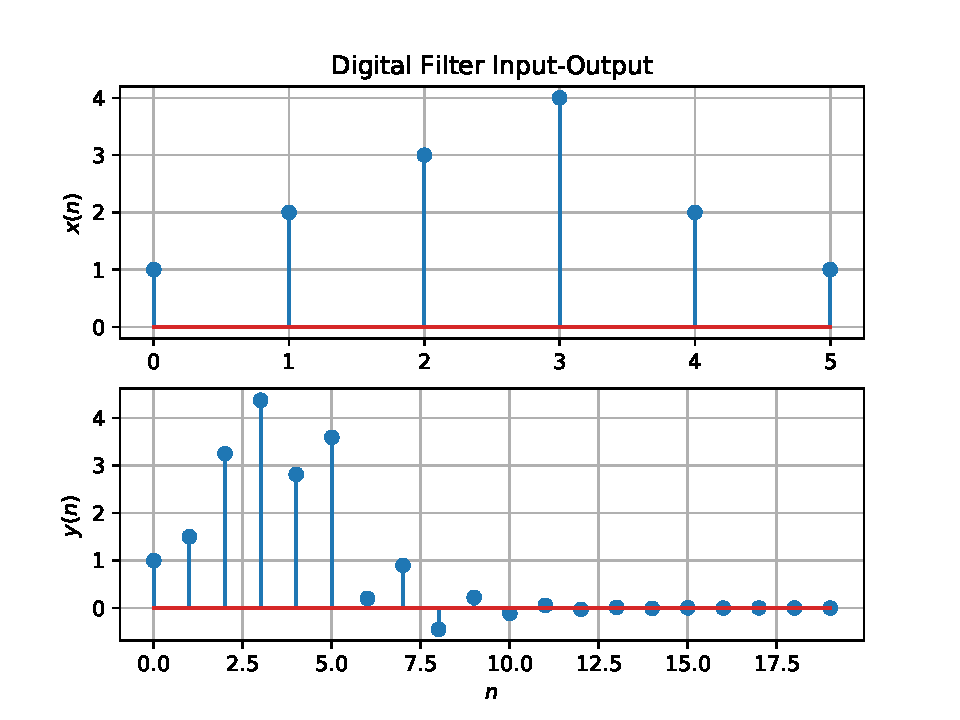
\includegraphics[width=\columnwidth]{./figs/xnyn}
\end{center}
\captionof{figure}{}
\label{fig:xnyn}	
\end{figure}

\item Repeat the above exercise using a C code. 
\solution
\begin{lstlisting}
wget https://github.com/TataSaiManoj/EE3900/blob/main/Assignment1/codes/toeplitz.c
\end{lstlisting}

\end{enumerate}

\section{Z - transform}
\begin{enumerate}[label=\thesection.\arabic*]
\item The $Z$-transform of $x(n)$ is defined as
%
\begin{equation}
\label{eq:z_trans}
X(z)={\mathcal {Z}}\{x(n)\}=\sum _{n=-\infty }^{\infty }x(n)z^{-n}
\end{equation}
%
Show that
\begin{equation}
\label{eq:shift1}
{\mathcal {Z}}\{x(n-1)\} = z^{-1}X(z)
\end{equation}
and find
\begin{equation}
	{\mathcal {Z}}\{x(n-k)\} 
\end{equation}
\solution From \eqref{eq:z_trans},
\begin{align}
{\mathcal {Z}}\{x(n-k)\} &=\sum _{n=-\infty }^{\infty }x(n - k)z^{-n}
\\
&=\sum _{n=-\infty }^{\infty }x(n)z^{-n-k} = z^{-k}\sum _{n=-\infty }^{\infty }x(n)z^{-n}
\end{align}
%
\begin{equation}
\label{eq:z_trans_shift}
	{\mathcal {Z}}\{x(n-k)\} = z^{-k}X(z)
\end{equation}

When $k = 1$, we get the equation 
\begin{equation}
		{\mathcal {Z}}\{x(n-1)\} = z^{-1}X(z)
\end{equation}

\item Obtain $X(z)$ for $x(n)$ defined in problem 
	\ref{eq:xn}.
\solution From \eqref{eq:z_trans}
\begin{align}
    X(z) &= \sum _{n=0 }^{5}x(n)z^{-n}\\
    &= x(0) + x(1)z^{-1} + \dots + x(5)z^{-5}\\
    &= 1 + 2z^{-1} + 3z^{-2} + 4z^{-3} + 2z^{-4} + z^{-5}
\end{align}

\item Find
%
\begin{equation}
H(z) = \frac{Y(z)}{X(z)}
\end{equation}
%
from  \eqref{eq:iir_filter} assuming that the $Z$-transform is a linear operation.
\\
\solution  Applying \eqref{eq:z_trans_shift} in \eqref{eq:iir_filter},
\begin{align}
Y(z) + \frac{1}{2}z^{-1}Y(z) &= X(z)+z^{-2}X(z)
\\
\implies \frac{Y(z)}{X(z)} &= \frac{1 + z^{-2}}{1 + \frac{1}{2}z^{-1}}
\label{eq:freq_resp}
\end{align}
%
\item Find the Z transform of 
\begin{equation}
\delta(n)
=
\begin{cases}
1 & n = 0
\\
0 & \text{otherwise}
\end{cases}
\end{equation}
and show that the $Z$-transform of
\begin{equation}
\label{eq:unit_step}
u(n)
=
\begin{cases}
1 & n \ge 0
\\
0 & \text{otherwise}
\end{cases}
\end{equation}
is
\begin{equation}
U(z) = \frac{1}{1-z^{-1}}, \quad \abs{z} > 1
\end{equation}
\solution It is easy to show that
\begin{equation}
\delta(n) \ztrans 1
\end{equation}
and from \eqref{eq:unit_step},
\begin{align}
U(z) &= \sum _{n= 0}^{\infty}z^{-n}
\\
&=\frac{1}{1-z^{-1}}, \quad \abs{z} > 1
\end{align}
using the formula for the sum of an infinite geometric progression.
%
\item Show that 
\begin{equation}
\label{eq:anun}
a^nu(n) \ztrans \frac{1}{1-az^{-1}} \quad \abs{z} > \abs{a}
\end{equation}

\solution
\begin{equation}
\label{eq:4.20}
x(n) = a^n u(n)
\end{equation}

\begin{equation}
\label{eq:4.21}
{\mathcal {Z}}\{x(n)\} = \sum  _{n = -\infty}^{\infty} a^{n}u(n)z^{-n}
\end{equation}

\begin{equation}
\label{eq:4.22}
{\mathcal {Z}}\{x(n)\} = \sum  _{n = 0}^{\infty} a^{n}z^{-n}
\end{equation}

\begin{equation}
\label{eq:4.23}
{\mathcal {Z}}\{x(n)\} = \sum _{n = 0}^{\infty} ({\frac{z}{a}})^{-n}
\end{equation}

\begin{equation}
    {\mathcal {Z}}\{x(n)\} =  \frac{1}{1 - az^{-1}}, \abs{z} > 1
\end{equation}
%
\item
Let
\begin{equation}
H\brak{e^{\text{\j} \omega}} = H\brak{z = e^{\text{\j} \omega}}.
\end{equation}
Plot $\abs{H\brak{e^{\text{\j} \omega}}}$.  Is it periodic? If so, find the period. $H(e^{\text{\j} \omega})$ is
known as the {\em Discrete Time Fourier Transform} (DTFT) of $x(n)$.\\
\solution The following code plots Fig. \ref{fig:dtft}.
\begin{align}
	\left|H\brak{e^{\text{\j}\omega}}\right| &= \left|\frac{1 + e^{-2\text{\j}\omega}}{1 + \frac{1}{2}e^{-\text{\j}\omega}}\right| \\
											 &= \sqrt{\frac{\brak{1 + \cos{2\omega}}^2 + \brak{\sin{2\omega}}^2}{\brak{1 + \frac{1}{2}\cos{\omega}}^2 + \brak{\frac{1}{2}\sin{\omega}}^2}} \\
											 &= \sqrt{\frac{2\brak{1 + \cos{2\omega}}}{\frac{5}{4} + \cos{\omega}}}				  		 
\end{align}
\begin{align}
									&= \sqrt{\frac{2\brak{2\cos^2{\omega}}}{\frac{5}{4} + \cos{\omega}}} \\
									&= \frac{4|\cos{\omega}|}{\sqrt{5 + 4\cos{\omega}}}
\end{align}
Thus,
\begin{align}
	H\brak{e^{\text{\j}\brak{\omega + 2\pi}}} &= \frac{4|\cos\brak{\omega + 2\pi}|}{\sqrt{5 + 4\cos\brak{\omega + 2\pi}}} \\
											   &= \frac{4|\cos{\omega}|}{\sqrt{5 + 4\cos{\omega}}} \\
											   &= H\brak{e^{\text{\j}\omega}}
\end{align}
So, the fundamental period is $2\pi$.

\begin{lstlisting}
wget https://github.com/TataSaiManoj/EE3900/blob/main/Assignment1/codes/dtft.py
\end{lstlisting}
\vspace{-5mm}
\begin{figure}[!ht]
\centering
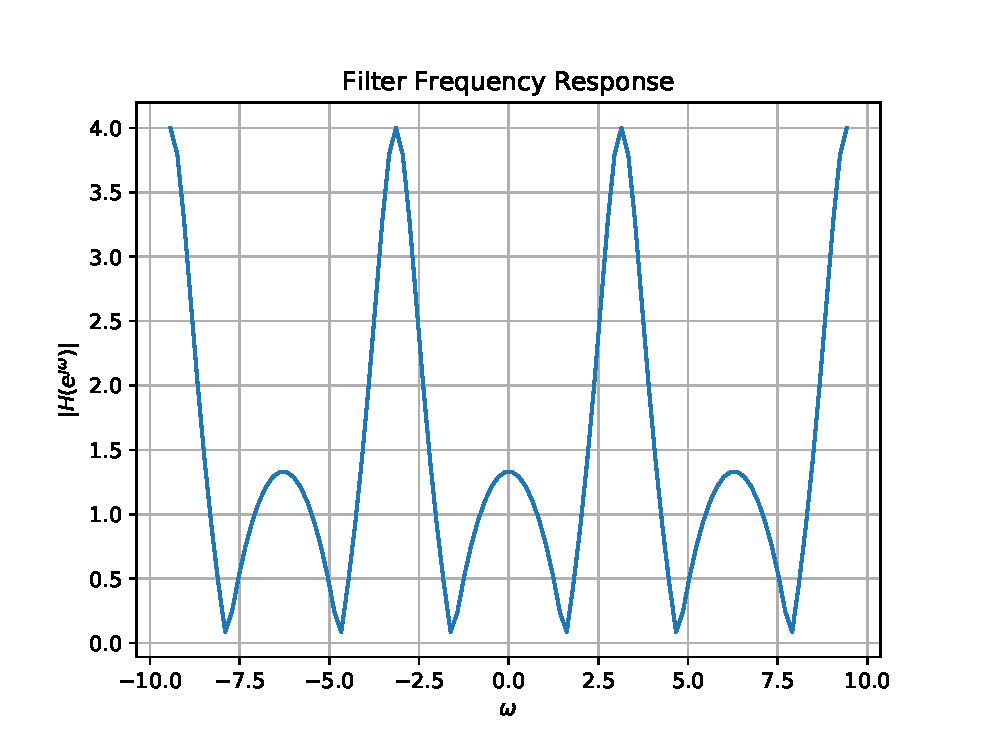
\includegraphics[width=\columnwidth]{./figs/dtft}
\caption{$\abs{H\brak{e^{\text{\j}\omega}}}$}
\label{fig:dtft}
\end{figure}
\item Express $h(n)$ in terms of $H\brak{e^{\text{\j} \omega}}$.
\\
\solution We have,
\begin{align}
	H(e^{\text{\j}\omega}) &= \sum_{k = -\infty}^{\infty}h(k)e^{-\text{\j}\omega k}
\end{align}

\begin{align}
	\int_{-\pi}^{\pi}e^{\text{\j}\omega(n - k)}d\omega =
	\begin{cases}
		2\pi & n = k \\
		0 & \textrm{otherwise}
	\end{cases}
\end{align}

% From the above equations, we have 
% \begin{align}
% 	&\frac{1}{2\pi}\int_{-\pi}^{\pi}H(e^{\text{\j}\omega})e^{j\omega n}d\omega \\
% 	&= \frac{1}{2\pi}\sum_{k = -\infty}^{\infty}\int_{-\pi}^{\pi}h(k)e^{\text{\j}\omega(n - k)}d\omega \\
% 	&= \frac{1}{2\pi}(2\pi h(n)) = h(n)
% \end{align}
% which is known as the Inverse Discrete Fourier Transform. 
% \begin{align}
%  	h(n) &= \frac{1}{2\pi}\int_{-\pi}^{\pi}H(e^{\text{\j}\omega})e^{\text{\j}\omega n}d\omega 
%  	\label{eq:idtft}
% \end{align}
% \end{enumerate}
\end{enumerate}

\section{Impulse Response}
\begin{enumerate}[label=\thesection.\arabic*]
	\item Using long division, 
find
		\begin{align}
			h(n), \quad n < 5
		\end{align}
		for H(z) in 
		\eqref{eq:freq_resp}.
\\

\solution Using the substitution $x := z^{-1}$, we perform long division.

\polylongdiv{1 + x^2}{1 + \frac{1}{2}x}\\
Thus,
\begin{align}
	H(z) &= -4 + 2z^{-1} + \frac{5}{1 + \frac{1}{2}z^{-1}} \\
		 &= -4 + 2z^{-1} + 5\sum_{n = 0}^{\infty}\brak{-\frac{1}{2}}^nz^{-n} \\
		 &= 1 - \frac{1}{2}z^{-1} + 5\sum_{n = 2}^{\infty}\brak{-\frac{1}{2}}^nz^{-n} \\
		 &= \sum_{n = 0}^{\infty}\brak{-\frac{1}{2}}^nz^{-n} + 4\sum_{n = 2}^{\infty}\brak{-\frac{1}{2}}^nz^{-n} \\
		 &= \sum_{n = -\infty}^{\infty}u(n)\brak{-\frac{1}{2}}^nz^{-n} + \nonumber \\
		 &\sum_{n = -\infty}^{\infty}u(n - 2)\brak{-\frac{1}{2}}^{n - 2}z^{-n}
\end{align}
Therefore, from \eqref{eq:z_trans}, 
\begin{align}
	h(n) = \brak{-\frac{1}{2}}^{n}u(n) + \brak{-\frac{1}{2}}^{n-2}u(n-2)
\end{align}

\item \label{prob:impulse_resp}
Find an expression for $h(n)$ using $H(z)$, given that 
%in Problem \ref{eq:ztransab} and \eqref{eq:anun}, given that
\begin{equation}
\label{eq:impulse_resp}
h(n) \ztrans H(z)
\end{equation}
and there is a one to one relationship between $h(n)$ and $H(z)$. $h(n)$ is known as the {\em impulse response} of the
system defined by \eqref{eq:iir_filter}.
\\
\solution From \eqref{eq:freq_resp},
\begin{align}
H(z) &= \frac{1}{1 + \frac{1}{2}z^{-1}} + \frac{ z^{-2}}{1 + \frac{1}{2}z^{-1}}
\\
\implies h(n) &= \brak{-\frac{1}{2}}^{n}u(n) + \brak{-\frac{1}{2}}^{n-2}u(n-2)
\end{align}
using \eqref{eq:anun} and \eqref{eq:z_trans_shift}.
\item Sketch $h(n)$. Is it bounded? Justify theoretically.
\\
\solution The following code plots Fig. \ref{fig:hn}.
\begin{lstlisting}
wget https://raw.githubusercontent.com/gadepall/EE1310/master/filter/codes/hn.py
\end{lstlisting}
\vspace{-5mm}
\begin{figure}[!ht]
\centering
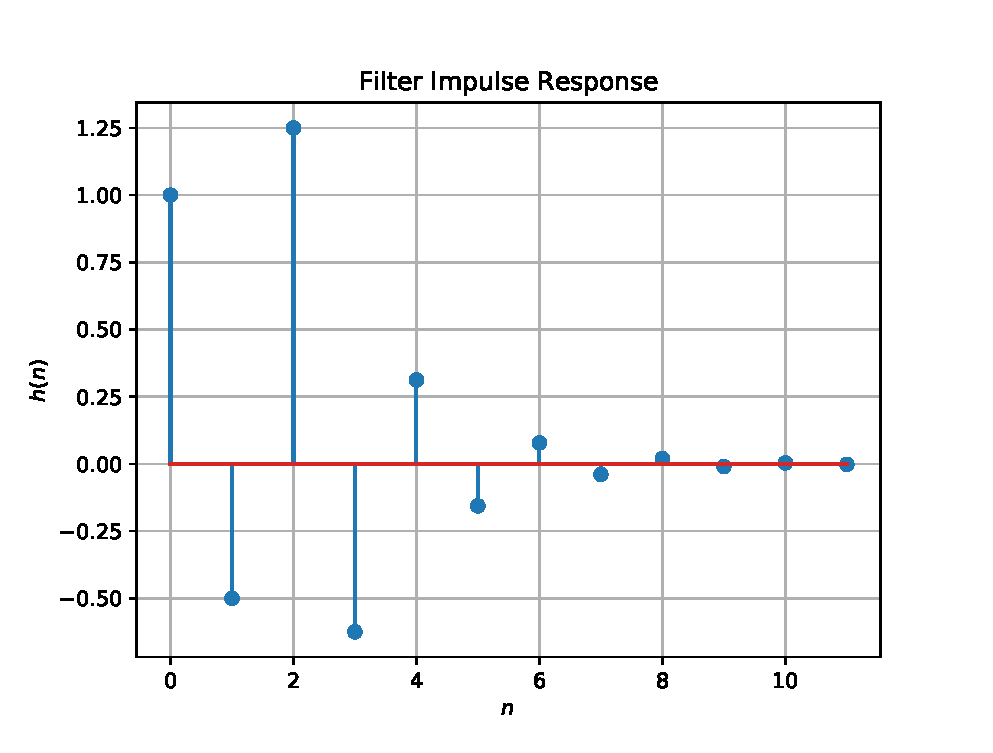
\includegraphics[width=\columnwidth]{./figs/hn}
\caption{$h(n)$ as the inverse of $H(z)$}
\label{fig:hn}
\end{figure}
From the Fig. \ref{fig:hn} we can see that $h(n)$ is bounded.
%
\item Convergent? Justify using the ratio test.
\\
\solution
For large $n$, we see that 
\begin{align}
	h(n) &= \brak{-\frac{1}{2}}^n + \brak{-\frac{1}{2}}^{n - 2} \\
		 &= \brak{-\frac{1}{2}}^{n}\brak{4 + 1} = 5\brak{-\frac{1}{2}}^n \\
		 &\implies \left|\frac{h(n + 1)}{h(n)}\right| = \frac{1}{2}
\end{align}
and therefore, $\lim_{n \to \infty}\left|\frac{h(n + 1)}{h(n)}\right| = \frac{1}{2} < 1$. Hence, we see that $h(n)$ converges.
\item The system with $h(n)$ is defined to be stable if
\begin{equation}
\sum_{n=-\infty}^{\infty}h(n) < \infty
\end{equation}
Is the system defined by \eqref{eq:iir_filter} stable for the impulse response in \eqref{eq:impulse_resp}?
\\
\solution
Note that
\begin{align}
	\sum_{n = -\infty}^{\infty}h\brak{n} &= \sum_{n = -\infty}^{\infty}
	\brak{-\frac{1}{2}}^nu\brak{n} + \\ &\brak{-\frac{1}{2}}^{n - 2}u\brak{n - 2} \\
										 &= 2\brak{\frac{1}{1 + \frac{1}{2}}} = \frac{4}{3}
\end{align}

% \begin{align}
% 	\sum_{n = -\infty}^{\infty}h\brak{n} < {\infty}
% \end{align}
Thus, the given system is stable.

%
\item Verify the above result using a python code.
\\
%
\item 
Compute and sketch $h(n)$ using 
\begin{equation}
\label{eq:iir_filter_h}
h(n) + \frac{1}{2}h(n-1) = \delta(n) + \delta(n-2), 
\end{equation}
%
This is the definition of $h(n)$.
\\
\solution The following code plots Fig. \ref{fig:hndef}. Note that this is the same as Fig. 
\ref{fig:hn}. 
%
\begin{lstlisting}
wget https://raw.githubusercontent.com/gadepall/EE1310/master/filter/codes/hndef.py
\end{lstlisting}
\begin{figure}[!ht]
\centering
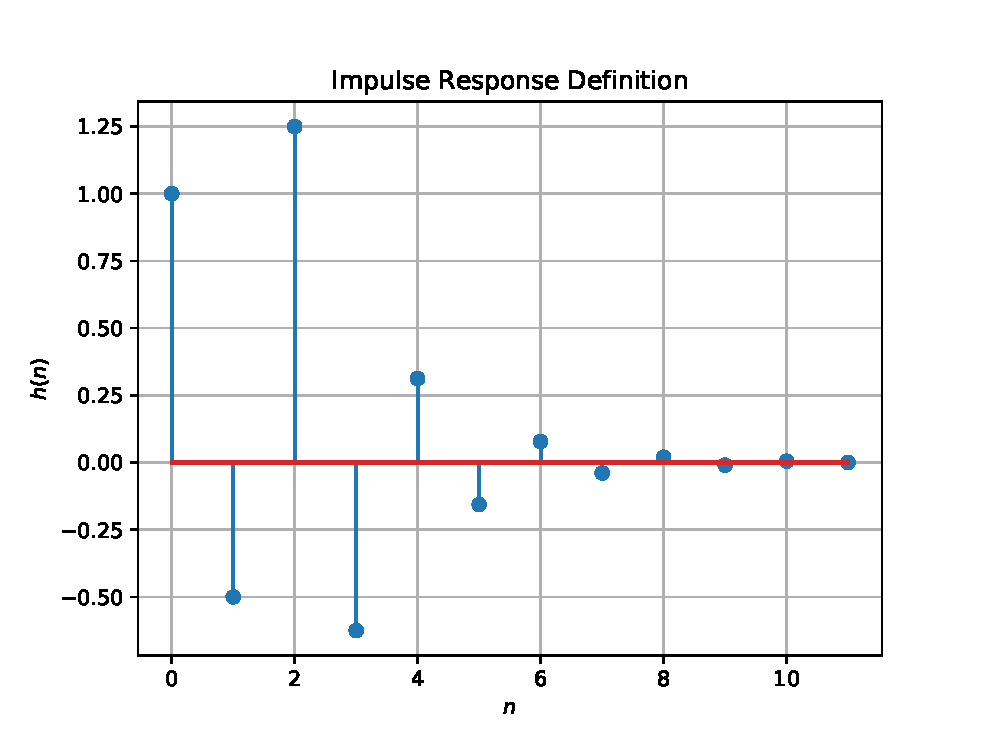
\includegraphics[width=\columnwidth]{./figs/hndef}
\caption{$h(n)$ from the definition}
\label{fig:hndef}
\end{figure}
%
\item Compute 
%
\begin{equation}
\label{eq:convolution}
y(n) = x(n)*h(n) = \sum_{n=-\infty}^{\infty}x(k)h(n-k)
\end{equation}
%
Comment. The operation in \eqref{eq:convolution} is known as
{\em convolution}.
%
\\
\solution The following code plots Fig. \ref{fig:ynconv}. Note that this is the same as 
$y(n)$ in  Fig. 
\ref{fig:xnyn}. 
%
\begin{lstlisting}
wget https://raw.githubusercontent.com/gadepall/EE1310/master/filter/codes/ynconv.py
\end{lstlisting}

\begin{figure}[!ht]
\centering
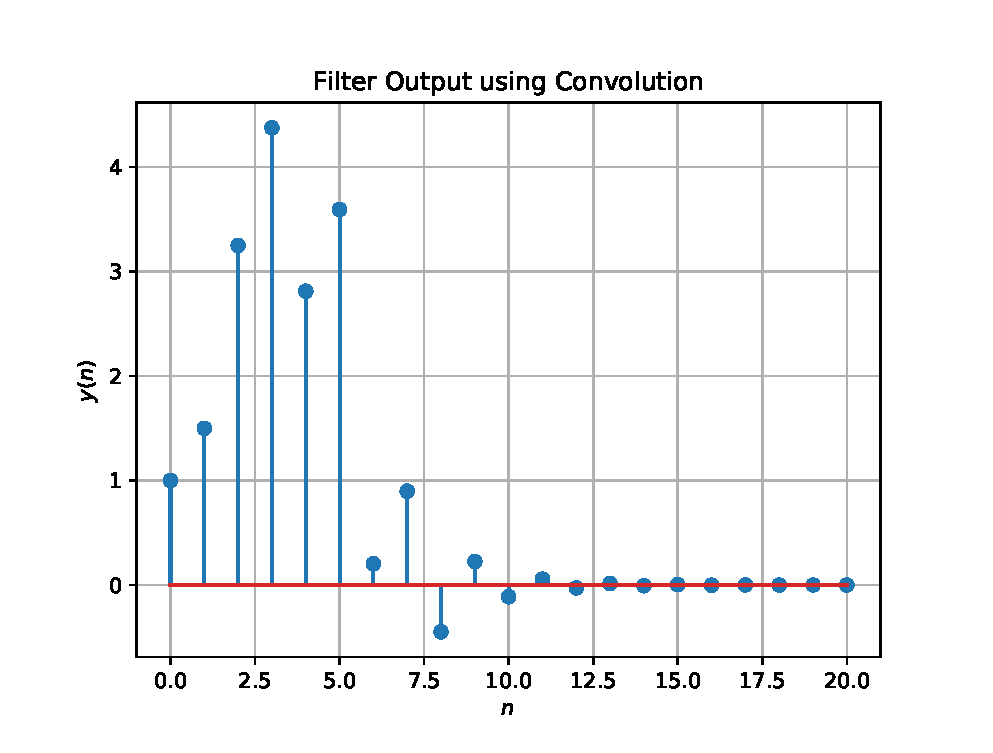
\includegraphics[width=\columnwidth]{./figs/ynconv}
\caption{$y(n)$ from the definition of convolution}
\label{fig:ynconv}
\end{figure}
\item Express the above convolution using a Toeplitz matrix.
\\
\solution We use Toeplitz matrices for convolution
\begin{align}
	\mtx{y} &= \mtx{x} \circledast \mtx{h}\\
	\mtx{y} &= 
	\begin{pmatrix}
		h_1 & 0 & . & . & . & 0 \\
		h_2 & h_1 & . & . & . & 0 \\
		h_3 & h_2 & h_1 & . & . & 0 \\
		. & . & . & . & . & . \\
		0 & . & . & h_3 & h_2 & h_1 \\
		0 & . & . & . & h_2 & h_1 \\
		0 & . & . & . & 0 & h_1
	\end{pmatrix}
	\begin{pmatrix}
		x_1 \\ x_2 \\ \vdots \\ x_n
	\end{pmatrix}
\end{align}
\item Show that
\begin{equation}
y(n) =  \sum_{n=-\infty}^{\infty}x(n-k)h(k)
\end{equation}
\\
\solution 
From \eqref{eq:convolution}, we substitute $k := n - k$ to get
\begin{align}
y\brak{n} &= \sum_{k=-\infty}^{\infty}x\brak{k}h\brak{n - k} \\
		  &= \sum_{n - k=-\infty}^{\infty}x\brak{n - k}h\brak{k} \\
		  &= \sum_{k=-\infty}^{\infty}x\brak{n - k}h\brak{k}
\end{align}
\end{enumerate}

%%%%% Section - 6 : DFT starts here %%%%
\section{DFT}
\begin{enumerate}[label=\thesection.\arabic*]
\item
Compute
\begin{equation}
X(k) \define \sum _{n=0}^{N-1}x(n) e^{-\text{\j}2\pi kn/N}, \quad k = 0,1,\dots, N-1
\end{equation}
and $H(k)$ using $h(n)$.

\solution
Run the following codes to compute $X(k)$ and $H(k)$.
\begin{lstlisting}
wget https://raw.githubusercontent.com/TataSaiManoj/EE3900/blob/main/Assignment1/codes/6_1_X(k).py
\end{lstlisting}
\begin{lstlisting}
wget https://raw.githubusercontent.com/TataSaiManoj/EE3900/blob/main/Assignment1/codes/6_1_H(k).py
\end{lstlisting}

\item Compute 
\begin{equation}
Y(k) = X(k)H(k)
\end{equation}
\solution
Run the following code to compute $Y(k)$.
\begin{lstlisting}
wget https://raw.githubusercontent.com/TataSaiManoj/EE3900/blob/main/Assignment1/codes/6_2.py
\end{lstlisting}

\item Compute
\begin{equation}
 y\brak{n}={\frac {1}{N}}\sum _{k=0}^{N-1}Y\brak{k}\cdot e^{\text{\j} 2\pi kn/N},\quad n = 0,1,\dots, N-1
\end{equation}
\\
\solution The following code plots Fig. \ref{fig:ynconv}. Note that this is the same as 
$y(n)$ in  Fig. 
\ref{fig:xnyn}. 
%
\begin{lstlisting}
wget https://raw.githubusercontent.com/TataSaiManoj/EE3900/blob/main/Assignment1/codes/6_3_yndft.py
\end{lstlisting}

\item Repeat the previous exercise by computing $X(k), H(k)$ and $y(n)$ through FFT and 
IFFT.
\solution

\begin{lstlisting}
wget https://raw.githubusercontent.com/TataSaiManoj/EE3900/blob/main/Assignment1/codes/6_4.py
\end{lstlisting}

\begin{figure}
	\centering
	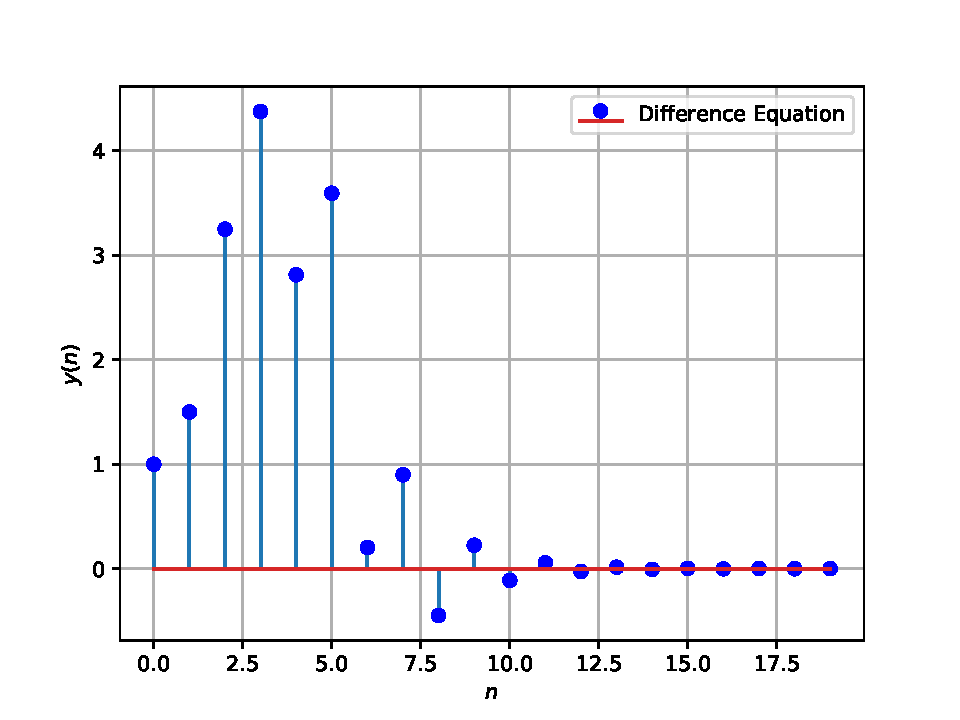
\includegraphics[width=0.8\columnwidth]{./figs/6_4_Diff.pdf}
	\caption{From the Difference Equation}	

	\centering
	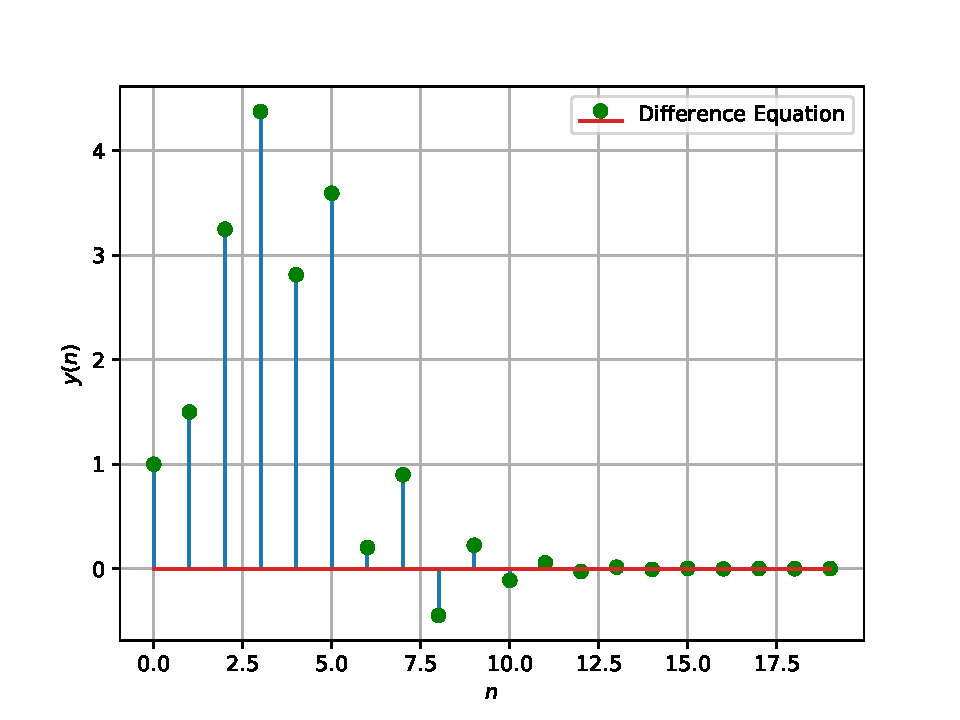
\includegraphics[width=0.8\columnwidth]{./figs/6_4_IDFT.pdf}
	\caption{From the IDFT}

	\centering
	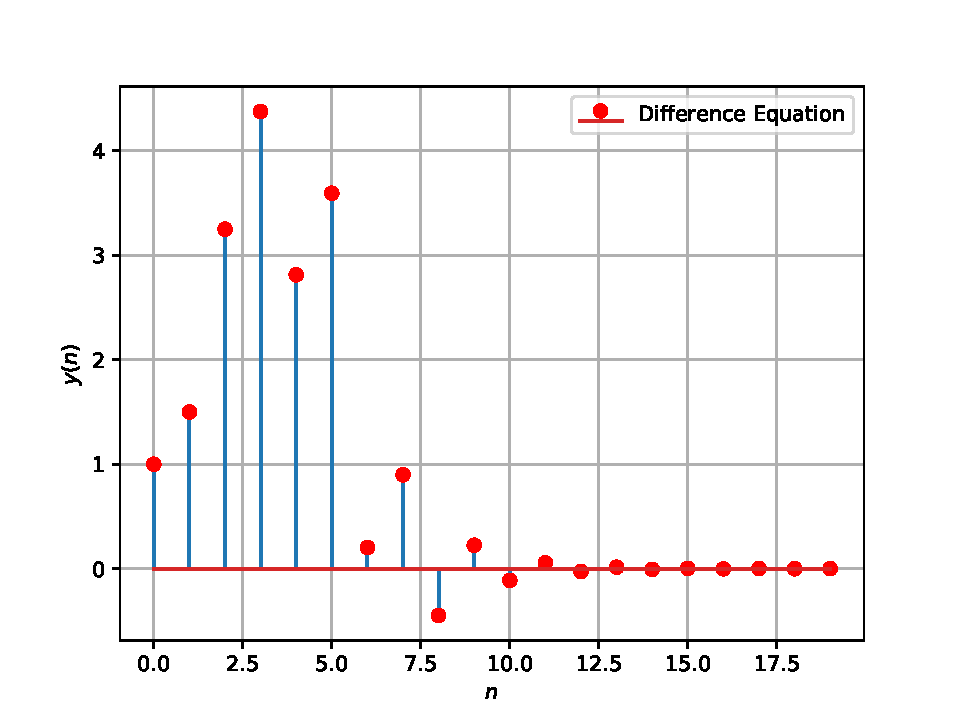
\includegraphics[width=0.8\columnwidth]{./figs/6_4_IFFT.pdf}
	\caption{From the IFFT}
\end{figure}
\end{enumerate}
\pagebreak

\section{FFT}
\begin{enumerate}[label=\thesection.\arabic*]
\item The DFT of $x(n)$ is given by
\begin{align}
        X(k) \triangleq \sum_{n=0}^{N-1} x(n) e^{-j 2 \pi k n / N}, \quad k=0,1, \ldots, N-1
\end{align}
\item Let 
	\begin{align}
W_{N} = e^{-j2\pi/N} 
	\end{align}
		Then the $N$-point {\em DFT matrix} is defined as 
	\begin{align}
		\vec{F}_{N} = \sbrak{W_{N}^{mn}}, \quad 0 \le m,n \le N-1 
	\end{align}
	where $W_{N}^{mn}$ are the elements of $\vec{F}_{N}$.
\item Let 
	\begin{align}
		\vec{I}_4 = \myvec{\vec{e}_4^{1} &\vec{e}_4^{2} &\vec{e}_4^{3} &\vec{e}_4^{4} }
	\end{align}
		be the $4\times 4$ identity matrix.  Then the 4 point {\em DFT permutation matrix} is defined as 
	\begin{align}
		\vec{P}_4 = \myvec{\vec{e}_4^{1} &\vec{e}_4^{3} &\vec{e}_4^{2} &\vec{e}_4^{4} }
	\end{align}
\item The 4 point {\em DFT diagonal matrix} is defined as 
	\begin{align}
		\vec{D}_4 = diag\myvec{W_{8}^{0} & W_{8}^{1} & W_{8}^{2} & W_{8}^{3}}
	\end{align}
\item Show that 
\begin{equation}
    W_{N}^{2}=W_{N/2}
\end{equation}

\solution
\begin{align}
	W_{N}^{2} &= \brak{e^{\brak{-j \cdot 2\pi N}}}^2\\
			  &= e^{-2\pi jN \cdot 2}\\
			  &= e^{-j \cdot \brak{\frac{2\pi}{N/2}}}\\
			  &= W_{N/2}		
\end{align}

%    \item Find $\vec{P}_6$.
%    \item Find $\vec{D}_3$.
    \item Show that 
\begin{equation}
	\vec{F}_{4}=
\begin{bmatrix}
	\vec{I}_{2} & \vec{D}_{2} \\
\vec{I}_{2} & -\vec{D}_{2}
\end{bmatrix}
\begin{bmatrix}
\vec{F}_{2} & 0 \\
0 & \vec{F}_{2}
\end{bmatrix}
\vec{P}_{4}
\end{equation}

\solution
\begin{align}
	&\mymat{\vec{I}_2 & \vec{D}_2 \\ \vec{I}_2 & -\vec{D}_2} \mymat{\vec{F}_2 & 0 \\ 0 & \vec{F}_2} \\
	= &\mymat{\vec{F}_2 & \vec{D}_2\vec{F}_2 \\ \vec{F}_2 & -\vec{D}_2\vec{F}_2} \\
	= &\mymat{\myvec{1&1\\1&-1} & \myvec{1&0\\0&-j}\myvec{1&1\\1&-1} \\ \myvec{1&1\\1&-1} & -\myvec{1&0\\0&-j}\myvec{1&1\\1&-1}}\\
	= &\mymat{1&1&1&1 \\ 1&-1&-j&j \\ 1&1&-1&-1 \\ 1&-1&j&-j}\\
	&\vec{P}_4 = \mymat{1&0&0&0 \\ 0&0&1&0 \\ 0&1&0&0 \\ 0&0&0&1}
\end{align}

\begin{align}
	&\mymat{1&1&1&1 \\ 1&-1&-j&j \\ 1&1&-1&-1 \\ 1&-1&j&-j} \mymat{1&0&0&0 \\ 0&0&1&0 \\ 0&1&0&0 \\ 0&0&0&1}\\
	&= \mymat{1 & 1 & 1 & 1 \\ 1 & -\text{\j} & -1 & \text{\j} \\ 1 & -1 & 1 & -1 \\ 1 & \text{\j} & -1 & -\text{\j}} \\
	&= \mymat{W_4^0 & W_4^0 & W_4^0 & W_4^0 \\ W_4^0 & W_4^1 & W_4^2 & W_4^3 \\ W_4^0 & W_4^2 & W_4^4 & W_4^6 \\ W_4^0 & W_4^3 & W_4^6 & W_4^9} \\
	&= \vec{F}_4
\end{align}

\item Show that 
\begin{equation}
\vec{F}_{N}=
\begin{bmatrix}
\vec{I}_{N/2} & \vec{D}_{N/2} \\
\vec{I}_{N/2} & -\vec{D}_{N/2}
\end{bmatrix}
\begin{bmatrix}
\vec{F}_{N/2} & 0 \\
0 & \vec{F}_{N/2}
\end{bmatrix}
\vec{P}_{N}
\end{equation}

\solution
\begin{align}
	&\mymat{\vec{I}_{N/2} & \vec{D}_{N/2} \\ \vec{I}_{N/2} & -\vec{D}_{N/2}} \mymat{\vec{F}_{N/2} & 0 \\ 0 & \vec{F}_{N/2}} \\
	&= \mymat{\vec{F}_{N/2} & \vec{D}_{N/2}\vec{F}_{N/2} \\ \vec{F}_{N/2} & -\vec{D}_{N/2}\vec{F}_{N/2}} 
\end{align}

\begin{equation}
	\vec{D}_{N/2} = \mymat{{W}_N & \cdots & 0 \\ \vdots & \ddots & \vdots \\ 0 & \cdots & {W}_{N}^{N/2 + 1}}
\end{equation}

\begin{equation}
	\vec{F}_{N/2} = \mymat{{W}_N^{0} & \cdots & {W}_{N}^0 \\ \vdots & \ddots & \vdots \\ {W}_{N/2}^{N/2 - 1} {W}_{N}^{0}& \cdots& {W}_{N/2}^{(N/2 - 1)^2}}
\end{equation}

Thus
\begin{align}
	\brak{\vec{D}_{N/2}\vec{F}_{N/2}}_{ij} &= W_N^i W_{N/2}^{ij} \\
	&= W_N^i {W_N^{2}}^{ij} \\
	&= W_N^{i(2j + 1)}
\end{align}
where $i, j = 0, \ldots, N/2 - 1$

$\vec{D}_{N/2}\vec{F}_{N/2}$ forms the first $N/2$ rows of the odd columns of $\vec{F}_N$

\begin{align}
	W_N^{(i + N/2)(2j + 1)} &= e^{\brak{-j \frac{2\pi}{N} (2j + 1)(i + \frac{N}{2})}} \\
	&= W_N^{i(2j + 1)}
\end{align}

The remaining $N/2$ rows of $\vec{F}_N$ are the negative of the first $N/2$ rows of $\vec{F}_N$.

Now, for the even-indexed columns, we have \\

$\vec{F}_{N/2}$ forms the first $N/2$ rows of the even columns of $\vec{F}_N$.
The remaining $N/2$ rows of $\vec{F}_N$ are the same as the first $N/2$ rows of $\vec{F}_N$.

Therefore
\begin{align}
	\mymat{\vec{F}_{N/2} & \vec{D}_{N/2}\vec{F}_{N/2} \\ \vec{F}_{N/2} & -\vec{D}_{N/2}\vec{F}_{N/2}} = \vec{F}_N \vec{P}_N
\end{align}
where 
\begin{align}
	\vec{P}_N = \myvec{\vec{e}_N^1 & \vec{e}_N^3 & \cdots & \vec{e}_N^{N-1} & \vec{e}_N^2 & \vec{e}_N^4 & \cdots & \vec{e}_N^N}
\end{align}

Hence
\begin{align}
	\mymat{\vec{F}_{N/2} & \vec{D}_{N/2}\vec{F}_{N/2} \\ \vec{F}_{N/2} & -\vec{D}_{N/2}\vec{F}_{N/2}} \vec{P}_N = \vec{F}_N \vec{P}_N^2 = \vec{F}_N \\
	\vec{F}_N = \mymat{\vec{I}_{N/2} & \vec{D}_{N/2} \\ \vec{I}_{N/2} & -\vec{D}_{N/2}} \mymat{\vec{F}_{N/2} & 0 \\ 0 & \vec{F}_{N/2}} \vec{P}_N
\end{align}
where $N$ is a power of 2.

\vspace{0.5mm}
\item Find 
    \begin{align}
	     \vec{P}_4 \vec{x}
    \end{align}

\solution
\\
Let $\vec{x} = \myvec{x_1 & x_2 & x_3 & x_4}$

\begin{align}
	\vec{P}_4 \vec{x} &= \mymat{1&0&0&0 \\ 0&0&1&0 \\ 0&1&0&0 \\ 0&0&0&1} \mymat{x_1 \\ x_2 \\ x_3 \\ x_4} \\
	&= \mymat{x_1 \\ x_3 \\ x_2 \\ x_4}
\end{align}

\item Show that 
    \begin{align}
	    \vec{X} = \vec{F}_N \vec{x}
	    \label{eq:dft-mat-def}
    \end{align}
		where $\vec{x}, \vec{X}$ are the vector representations of $x(n), X(k)$ respectively.

\solution
\begin{align}
	X(k) &= \sum_{n=0}^{N-1} x(n) e^{-j 2 \pi k n / N}\\
	\vec{X} &= \mymat{\sum_{n=0}^{N-1} x(n) e^{-j 2 \pi  n (0) / N} \\ \vdots \\ \sum_{n=0}^{N-1} x(n) e^{-j 2 \pi  n (N-1) / N}} \\
	&= \mymat{x(0) + \cdots + x(N-1) \\ \vdots \\ x(0) + \cdots + x(N-1) e^{-j 2 \pi (N-1)^2 / N}} 
\end{align}
\begin{align}
		\vec{X} &= x(0) \mymat{1 \\ \vdots \\ 1} + \cdots + x(N-1)\mymat{1 \\ \vdots \\ e^{-j 2 \pi (N-1)^2 / N}} \\
		&= \mymat{1 & \cdots & 1 \\ \vdots & \ddots & \vdots \\ 1 & \cdots & e^{-j 2 \pi (N-1)^2 / N}} \mymat{x(0) \\ \vdots \\ x(N-1)} \\
		&= \vec{F}_N \vec{x}
\end{align}

\item Derive the following Step-by-step visualisation  of
8-point FFTs into 4-point FFTs and so on
\begin{equation}
\begin{bmatrix}
X(0) \\ 
X(1) \\ 
X(2) \\ 
X(3)
\end{bmatrix}
=
\begin{bmatrix}
X_{1}(0) \\ 
X_{1}(1)\\ 
X_{1}(2)\\
X_{1}(3)\\
\end{bmatrix}
+
\begin{bmatrix}
W^{0}_{8} & 0 & 0 & 0\\
0 & W^{1}_{8} & 0 & 0\\
0 & 0 & W^{2}_{8} & 0\\
0 & 0 & 0 & W^{3}_{8}
\end{bmatrix}
\begin{bmatrix}
X_{2}(0) \\ 
X_{2}(1) \\ 
X_{2}(2) \\
X_{2}(3)
\end{bmatrix}
\end{equation}
\begin{equation}
\begin{bmatrix}
X(4) \\ 
X(5) \\ 
X(6) \\ 
X(7)
\end{bmatrix}
=
\begin{bmatrix}
X_{1}(0) \\ 
X_{1}(1)\\ 
X_{1}(2)\\
X_{1}(3)\\
\end{bmatrix}
-
\begin{bmatrix}
W^{0}_{8} & 0 & 0 & 0\\
0 & W^{1}_{8} & 0 & 0\\
0 & 0 & W^{2}_{8} & 0\\
0 & 0 & 0 & W^{3}_{8}
\end{bmatrix}
\begin{bmatrix}
X_{2}(0) \\ 
X_{2}(1) \\ 
X_{2}(2) \\
X_{2}(3)
\end{bmatrix}
\end{equation}
4-point FFTs into 2-point FFTs
\begin{equation}
\begin{bmatrix}
X_{1}(0) \\ 
X_{1}(1)\\ 
\end{bmatrix}
=
\begin{bmatrix}
X_{3}(0) \\ 
X_{3}(1)\\ 
\end{bmatrix}
+
\begin{bmatrix}
W^{0}_{4} & 0\\
0 & W^{1}_{4}
\end{bmatrix}
\begin{bmatrix}
X_{4}(0) \\ 
X_{4}(1) \\ 
\end{bmatrix}
\end{equation}
\begin{equation}
\begin{bmatrix}
X_{1}(2) \\ 
X_{1}(3)\\ 
\end{bmatrix}
=
\begin{bmatrix}
X_{3}(0) \\ 
X_{3}(1)\\ 
\end{bmatrix}
-
\begin{bmatrix}
W^{0}_{4} & 0\\
0 & W^{1}_{4}
\end{bmatrix}
\begin{bmatrix}
X_{4}(0) \\ 
X_{4}(1) \\ 
\end{bmatrix}
\end{equation}
\begin{equation}
\begin{bmatrix}
X_{2}(0) \\ 
X_{2}(1)\\ 
\end{bmatrix}
=
\begin{bmatrix}
X_{5}(0) \\ 
X_{5}(1)\\ 
\end{bmatrix}
+
\begin{bmatrix}
W^{0}_{4} & 0\\
0 & W^{1}_{4}
\end{bmatrix}
\begin{bmatrix}
X_{6}(0) \\ 
X_{6}(1) \\ 
\end{bmatrix}
\end{equation}
\begin{equation}
\begin{bmatrix}
X_{2}(2) \\ 
X_{2}(3)\\ 
\end{bmatrix}
=
\begin{bmatrix}
X_{5}(0) \\ 
X_{5}(1)\\ 
\end{bmatrix}
-
\begin{bmatrix}
W^{0}_{4} & 0\\
0 & W^{1}_{4}
\end{bmatrix}
\begin{bmatrix}
X_{6}(0) \\ 
X_{6}(1) \\ 
\end{bmatrix}
\end{equation}
\begin{equation}
P_{8}
\begin{bmatrix}
x(0) \\ 
x(1) \\ 
x(2) \\ 
x(3) \\ 
x(4) \\ 
x(5) \\
x(6) \\
x(7)
\end{bmatrix}
 = 
\begin{bmatrix}
x(0) \\ 
x(2) \\ 
x(4) \\ 
x(6) \\
x(1) \\ 
x(3) \\ 
x(5) \\
x(7)
\end{bmatrix}
\end{equation}
\begin{equation}
P_{4}
\begin{bmatrix}
x(0) \\ 
x(2) \\ 
x(4) \\ 
x(6) \\
\end{bmatrix}
 = 
\begin{bmatrix}
x(0) \\ 
x(4) \\ 
x(2) \\
x(6)
\end{bmatrix}
\end{equation}
\begin{equation}
P_{4}
\begin{bmatrix}
x(1) \\ 
x(3) \\ 
x(5) \\
x(7)
\end{bmatrix}
 = 
\begin{bmatrix}
x(1) \\ 
x(5) \\ 
x(3) \\ 
x(7) \\
\end{bmatrix}
\end{equation}
Therefore,
\begin{equation}
\begin{bmatrix}
X_{3}(0) \\ 
X_{3}(1)\\ 
\end{bmatrix}
= F_{2}
\begin{bmatrix}
x(0) \\ 
x(4) \\ 
\end{bmatrix}
\end{equation}
\begin{equation}
\begin{bmatrix}
X_{4}(0) \\ 
X_{4}(1)\\ 
\end{bmatrix}
= F_{2}
\begin{bmatrix}
x(2) \\ 
x(6) \\ 
\end{bmatrix}
\end{equation}
\begin{equation}
\begin{bmatrix}
X_{5}(0) \\ 
X_{5}(1)\\ 
\end{bmatrix}
= F_{2}
\begin{bmatrix}
x(1) \\ 
x(5) \\ 
\end{bmatrix}
\end{equation}
\begin{equation}
\begin{bmatrix}
X_{6}(0) \\ 
X_{6}(1)\\ 
\end{bmatrix}
= F_{2}
\begin{bmatrix}
x(3) \\ 
x(7) \\ 
\end{bmatrix}
\end{equation}

\solution 
\\ We write out the values of performing an 8-point FFT on $\vec{x}$ as follows.
\begin{align}
	X(k) &= \sum_{n = 0}^{7}x(n)e^{-\frac{j2kn\pi}{8}} \\
		 &= \sum_{n = 0}^{3}\brak{x(2n)e^{-\frac{j2kn\pi}{4}} + e^{-\frac{j2k\pi}{8}}x(2n + 1)e^{-\frac{j2kn\pi}{4}}} \\
		 &= X_1(k) + e^{-\frac{j2k\pi}{4}}X_2(k) 
\end{align}

where $\vec{X}_1$ is the 4-point FFT of the even-numbered terms and $\vec{X}_2$ is the 4-point FFT of the odd numbered terms. Noticing that for $k \geq 4$,

\begin{align}
	X_1(k) &= X_1(k - 4) \\
	e^{-\frac{j2k\pi}{8}} &= -e^{-\frac{j2(k - 4)\pi}{8}}
\end{align}

We can now write out $X(k)$ in matrix form.
We also need to solve the two 4-point FFT terms so formed.

\begin{align}
	X_1(k) &= \sum_{n = 0}^{3}x_1(n)e^{-\frac{j2kn\pi}{8}} \\
		 &= \sum_{n = 0}^{1}\brak{x_1(2n)e^{-\frac{j2kn\pi}{4}}}\\
		 &+ \sum_{n = 0}^{1}\brak{e^{-\frac{j2k\pi}{8}}x_2(2n + 1)e^{-\frac{j2kn\pi}{4}}} \\
		 &= X_3(k) + e^{-\frac{j2k\pi}{4}}X_4(k) 
\end{align}

using $x_1(n) = x(2n)$ and $x_2(n) = x(2n + 1)$. Thus we can write the 2-point FFTs

\begin{align}
\begin{bmatrix}
X_{3}(0) \\ 
X_{3}(1)\\ 
\end{bmatrix}
= F_{2}
\begin{bmatrix}
x(0) \\ 
x(4) \\ 
\end{bmatrix} \\
\begin{bmatrix}
X_{4}(0) \\ 
X_{4}(1)\\ 
\end{bmatrix}
= F_{2}
\begin{bmatrix}
x(2) \\ 
x(6) \\ 
\end{bmatrix}
\end{align}
Using a similar idea for the terms $X_2$, 
\begin{align}
\begin{bmatrix}
X_{5}(0) \\ 
X_{5}(1)\\ 
\end{bmatrix}
= F_{2}
\begin{bmatrix}
x(1) \\ 
x(5) \\ 
\end{bmatrix} \\
\begin{bmatrix}
X_{6}(0) \\ 
X_{6}(1)\\ 
\end{bmatrix}
= F_{2}
\begin{bmatrix}
x(3) \\ 
x(7) \\ 
\end{bmatrix}
\end{align}

% But observe that from \eqref{eq:x-permute},

\begin{align}
	\vec{P}_8\vec{x} &= \myvec{\vec{x}_1\\\vec{x}_2} \\
	\vec{P}_4\vec{x}_1 &= \myvec{\vec{x}_3\\\vec{x}_4} \\ 
	\vec{P}_4\vec{x}_2 &= \myvec{\vec{x}_5\\\vec{x}_6}
\end{align}
where we define $x_3(k) = x(4k)$, $x_4(k) = x(4k + 2)$, $x_5(k) = x(4k + 1)$, and $x_6(k) = x(4k + 3)$ for $k = 0, 1$.

\item For 
    \begin{align}
	    \vec{x} = \myvec{1\\2\\3\\4\\2\\1}
        \label{eq:equation1}
    \end{align}
    compte the DFT  
		using 
	    \eqref{eq:dft-mat-def}

\solution
\\Download the following Python code that plots Fig. \ref{fig-7.11}.
\begin{lstlisting}
	7.11.py
\end{lstlisting}

\begin{figure}[!ht]
	\centering
	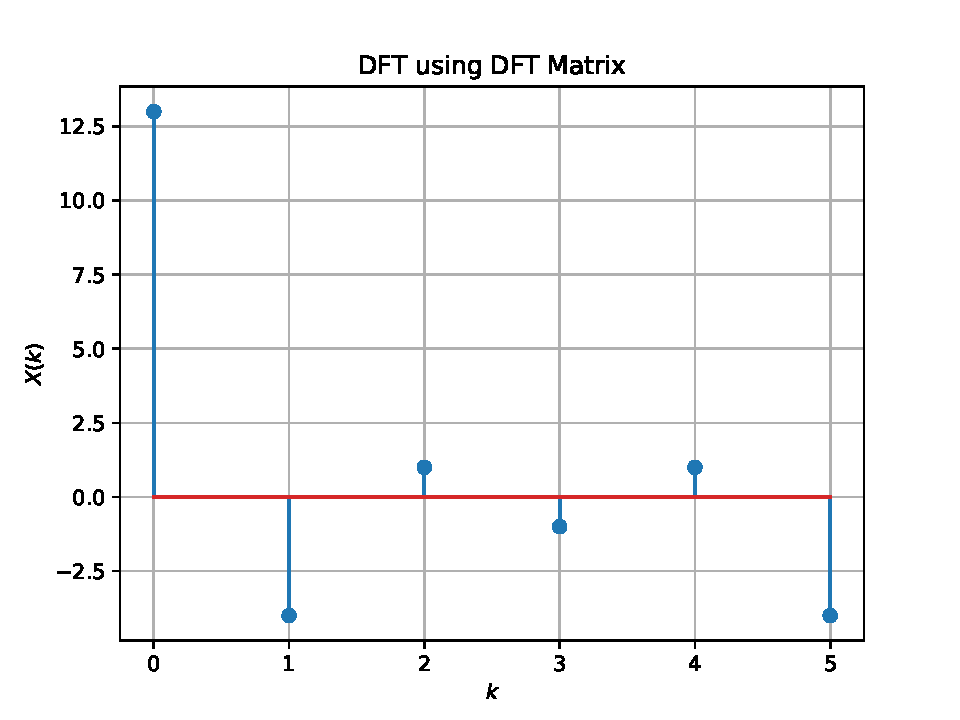
\includegraphics[width=\columnwidth]{./figs/7.11.pdf}
	\caption{Plot using DFT matrix}
	\label{fig-7.11}	
\end{figure}


\item Repeat the above exercise using the FFT
	after zero padding $\vec{x}$.

	\solution Download the following Python code that plots Fig. \ref{fig-7.12}.
	\vspace{1mm}
	\begin{lstlisting}
		7.12.py
	\end{lstlisting}

	\begin{figure}[!ht]
		\centering
		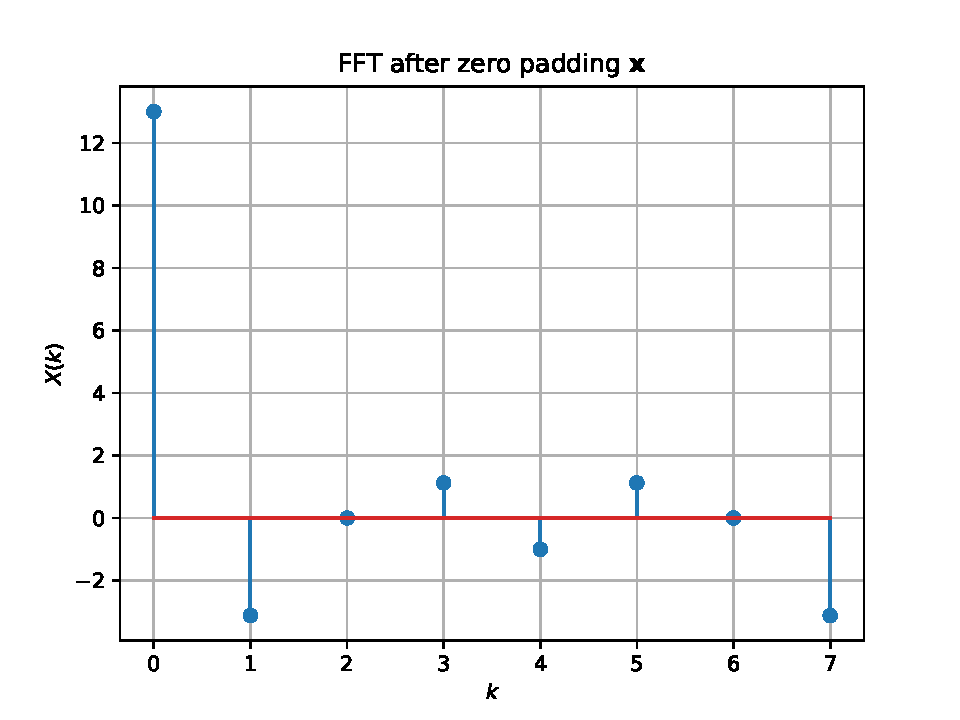
\includegraphics[width=\columnwidth]{./figs/7.12.pdf}
		\caption{Plot of FFT with zero padding}
		\label{fig-7.12}	
	\end{figure}

%	    \eqref{eq:fft-mat-def}
\item Write a C program to compute the 8-point FFT. 
\solution
\\Download the following C code that generates the values of $X(k)$ using $8$-point FFT

\begin{lstlisting}
	8pointFFT.c
\end{lstlisting}

Download the following Python code that generates the plot of $8$-point FFT from the C code

\begin{lstlisting}
	7_13.py
\end{lstlisting}

\begin{figure}[!ht]
	\centering
	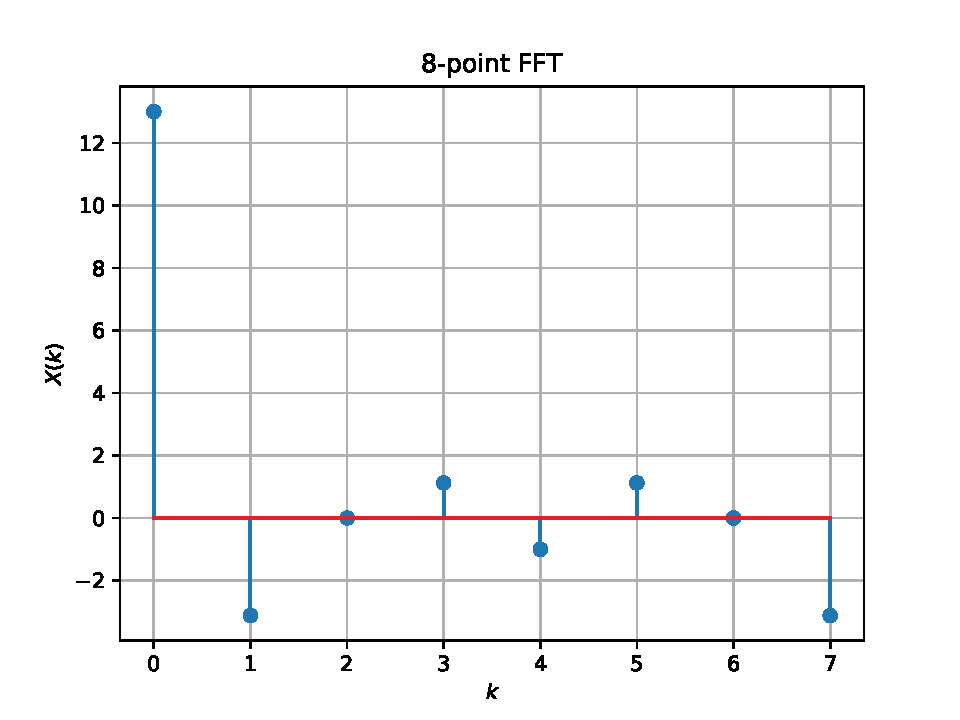
\includegraphics[width=\columnwidth]{./figs/7.13.pdf}
	\caption{Plot of FFT using C}
	\label{fig-7.13}	
\end{figure}

\item Time complexity comparison of FFT and \\convolution\\
\solution
\\The following C code notes the running times of FFT and convolution
and the python code plots the results.

\begin{lstlisting}
	8pointFFT_times.c
	7.14.py
\end{lstlisting}

\begin{figure}[!ht]
	\centering
	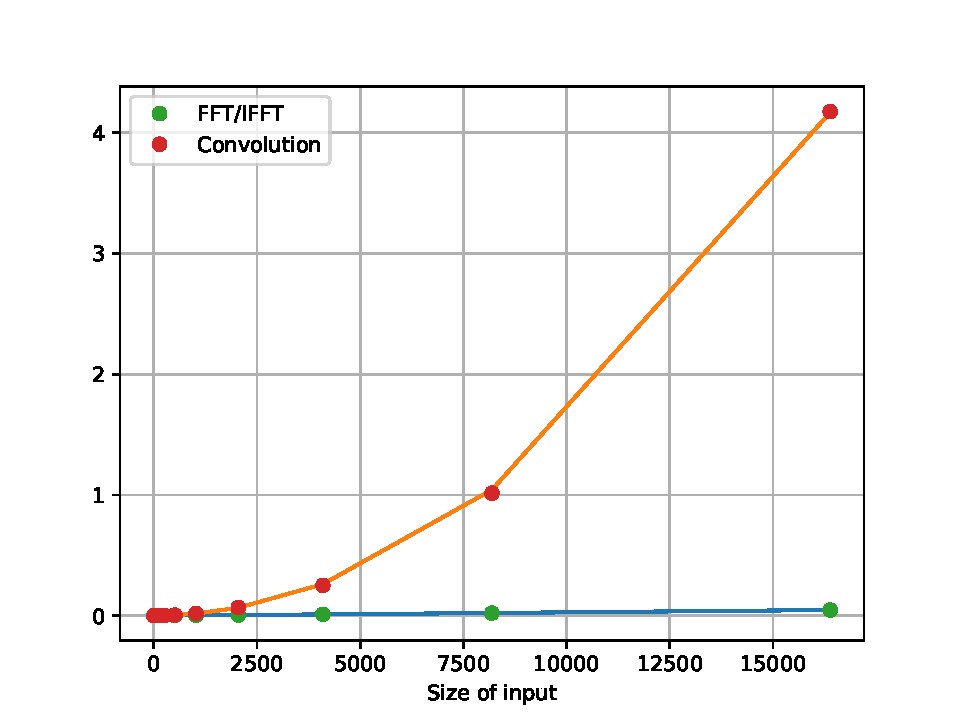
\includegraphics[width=\columnwidth]{./figs/7.14.pdf}
	\label{fig-7.14}
\end{figure}
\end{enumerate}

\pagebreak
\section{Exercises}

Answer the following questions by looking at the python code in Problem \ref{prob:output}

\begin{enumerate}[label=\thesection.\arabic*]
\item The command

\begin{lstlisting}
output_signal = signal.lfilter(b, a, input_signal)
\end{lstlisting}

in Problem \ref{prob:output} is executed through the following difference equation
\begin{equation}
	\label{eq:iir_filter_gen}
	\sum _{m=0}^{M}a\brak{m}y\brak{n-m}=\sum _{k=0}^{N}b\brak{k}x\brak{n-k}
\end{equation}
where the input signal is $x(n)$ and the output signal is $y(n)$ with initial values all 0. Replace \textbf{signal.filtfilt} with your own routine and verify.

\solution On taking the $Z$-transform on both sides of the difference equation
\begin{align}
	\sum _{m=0}^{M}a\brak{m} z^{-m} Y(z) &= \sum _{k=0}^{N}b\brak{k} z^{-k} X(z) \\
	\implies H(z) = \frac{Y(z)}{X(z)} &= \frac{\sum _{k=0}^{N}b\brak{k} z^{-k}}{\sum _{m=0}^{M}a\brak{m} z^{-m}}
\end{align}

For obtaining the discrete Fourier transform, put $z = j \frac{2\pi i}{I}$ where $I$ is the length of the input signal and $i = 0, 1, \ldots, I-1$

Download the following Python code 
\begin{lstlisting}
	8_1.py
\end{lstlisting}

\item Repeat all the exercises in the previous sections for the above $a$ and $b$	

\solution
Using the previous routine, we can find the output signal using FFT/IFFT and also plot $h(n)$ using the following Python code
\begin{lstlisting}
	8_2.py
\end{lstlisting}


\begin{figure}[htp]
	\centering
	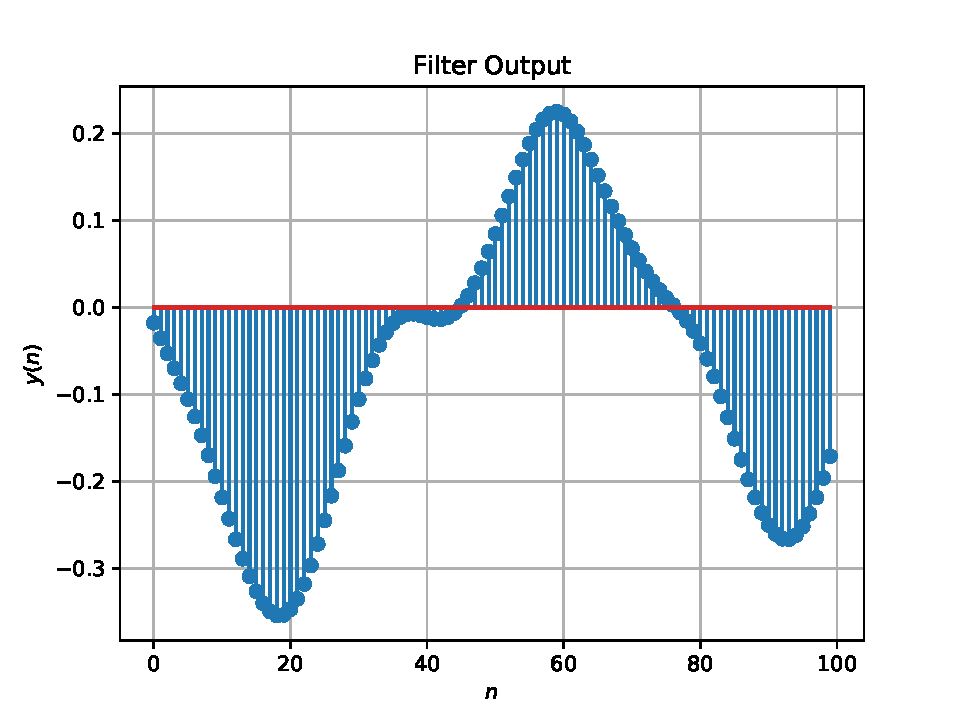
\includegraphics[width=\columnwidth]{./figs/8.2_y(n).pdf}
	\caption{Plot of $y(n)$}
	\label{fig-8.2_y(n)}
\end{figure}

\begin{figure}[htp]
	\centering
	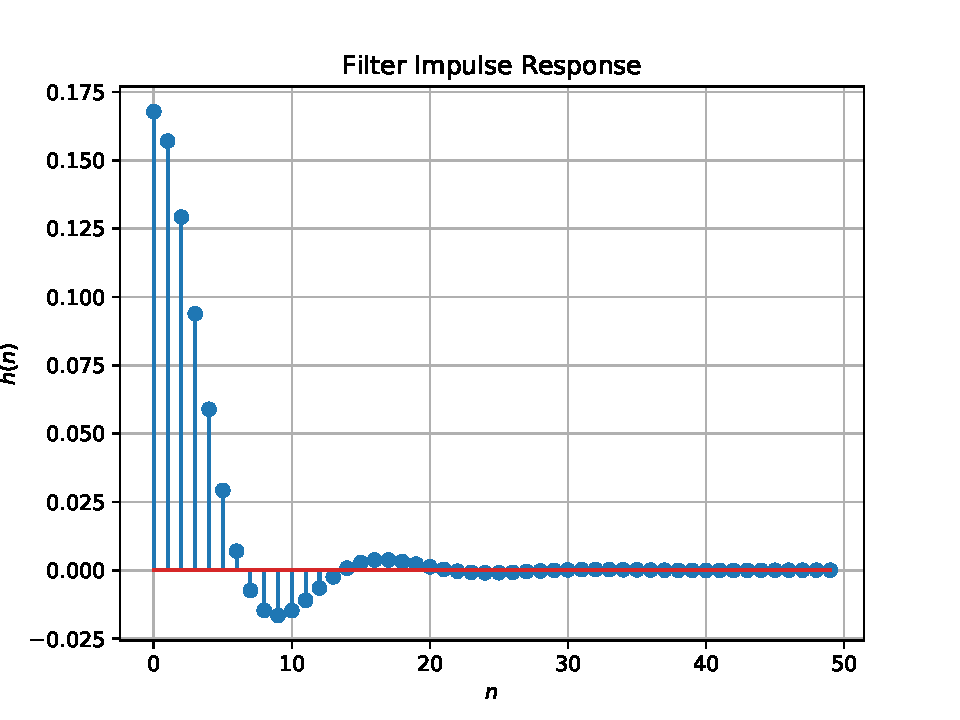
\includegraphics[width=\columnwidth]{./figs/8.2_h(n).pdf}
	\caption{Plot of $h(n)$}
	\label{fig-8.2_h(n)}	
\end{figure}


\item What is the sampling frequency of the input signal?

\solution The sampling frequency of the input signal is 44.1 kHz

\item What is the type, order and cutoff frequency of the above Butterworth filter?

\solution 

It is a low-pass filter of order 4. The cutoff frequency is 4000Hz.
\pagebreak

\item Modify the code with different input parameters to get the best possible output.

\solution

Best possible output is obtained when order is 10 and cutoff frequency of 3000Hz.

\end{enumerate}

\end{document}


